\documentclass[10pt,twoside,english,a4paper]{article}
\usepackage[utf8]{inputenc}
\usepackage{graphicx}
\usepackage{url} 
\usepackage{hyperref} 
\usepackage{cite}
%\usepackage{times}
\pagestyle{headings}

\title{Improving computer science and software 
engineering education in cyberlearning 
environments through understanding UI and UX design
\thanks{Semestrálny projekt v predmete Metódy inžinierskej práce,
 ak. rok 2020/21, vedenie: Martin Sabo}}

\author{Márk Bartalos \\[2pt]
        \small{Slovak University of Technology in Bratislava}\\
        \small{Faculty of Informatics and Information Technologies}\\
        \small{\texttt{xbartalosm@stuba.sk}}
}

\date{\small 30. september 2020}


\begin{document}

\maketitle

\begin{abstract}
    In our day and age cyberlearning for computer science and software engineering education has become more popular than ever. 
The article will be about how understanding UI and UX design principles can serve as a basis for future improvements in teaching
these fields. My goal is to understand UI/UX design techniques to be able to identify the problems with currently 
implemented cyberlearning environment designs. The identified problems then could be used to improve already existing environments.
Knowledge of these problems would be greatly beneficial in the design and development of new, learning focused, student 
oriented cyberlearning environments for computer science and software engineering students.
\end{abstract}



\section{Introduction}
We speak about distance learning for about two centuries \cite{moore_2011_elearning} 

% Motivujte čitateľa a vysvetlite, o čom píšete. Úvod sa väčšinou nedelí na časti.

% Uveďte explicitne štruktúru článku. Tu je nejaký príklad.
% Základný problém, ktorý bol naznačený v úvode, je podrobnejšie vysvetlený v časti~\ref{nejaka}.
% Dôležité súvislosti sú uvedené v častiach~\ref{dolezita} a~\ref{dolezitejsia}.
% Záverečné poznámky prináša časť~\ref{zaver}.

\section{Graphics}

\begin{figure}
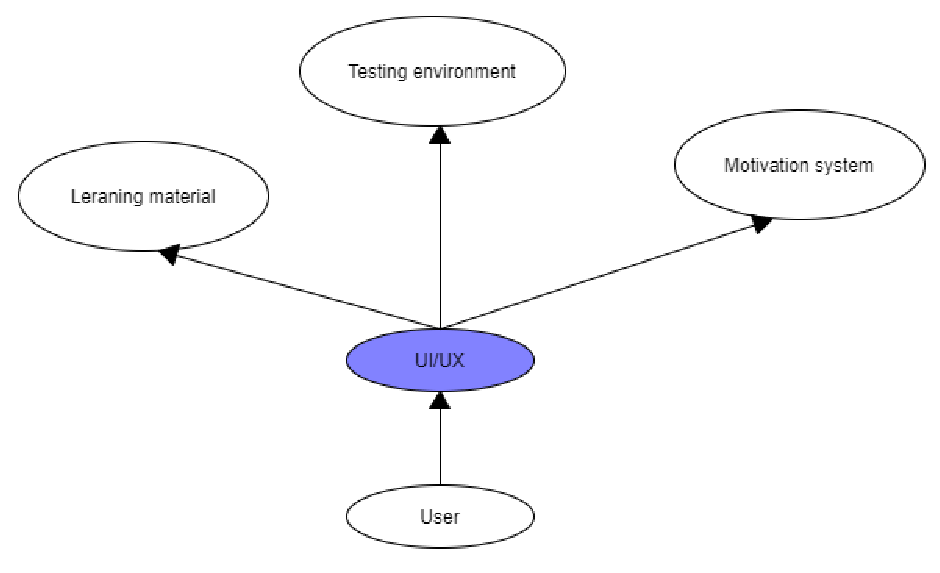
\includegraphics[width=0.75\textwidth]{images/diagram-crop.pdf}
\end{figure}

\begin{figure}
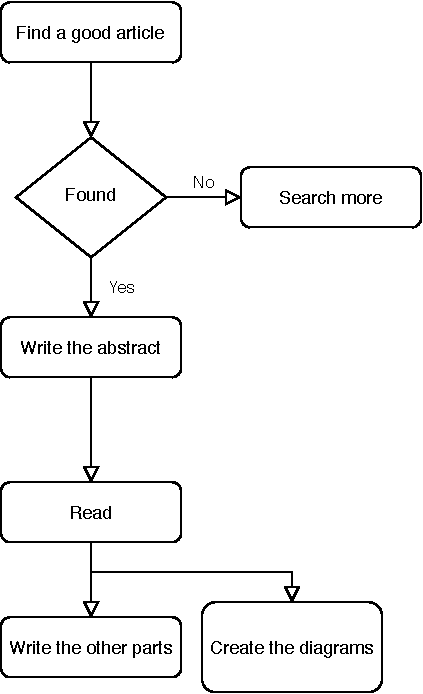
\includegraphics[width=0.75\textwidth]{images/flowchart-crop.pdf}
\end{figure}
% \section{Nejaká časť} \label{nejaka}

% Z obr.~\ref{f:rozhod} je všetko jasné. 

% \begin{figure*}[tbh]
% \centering
% %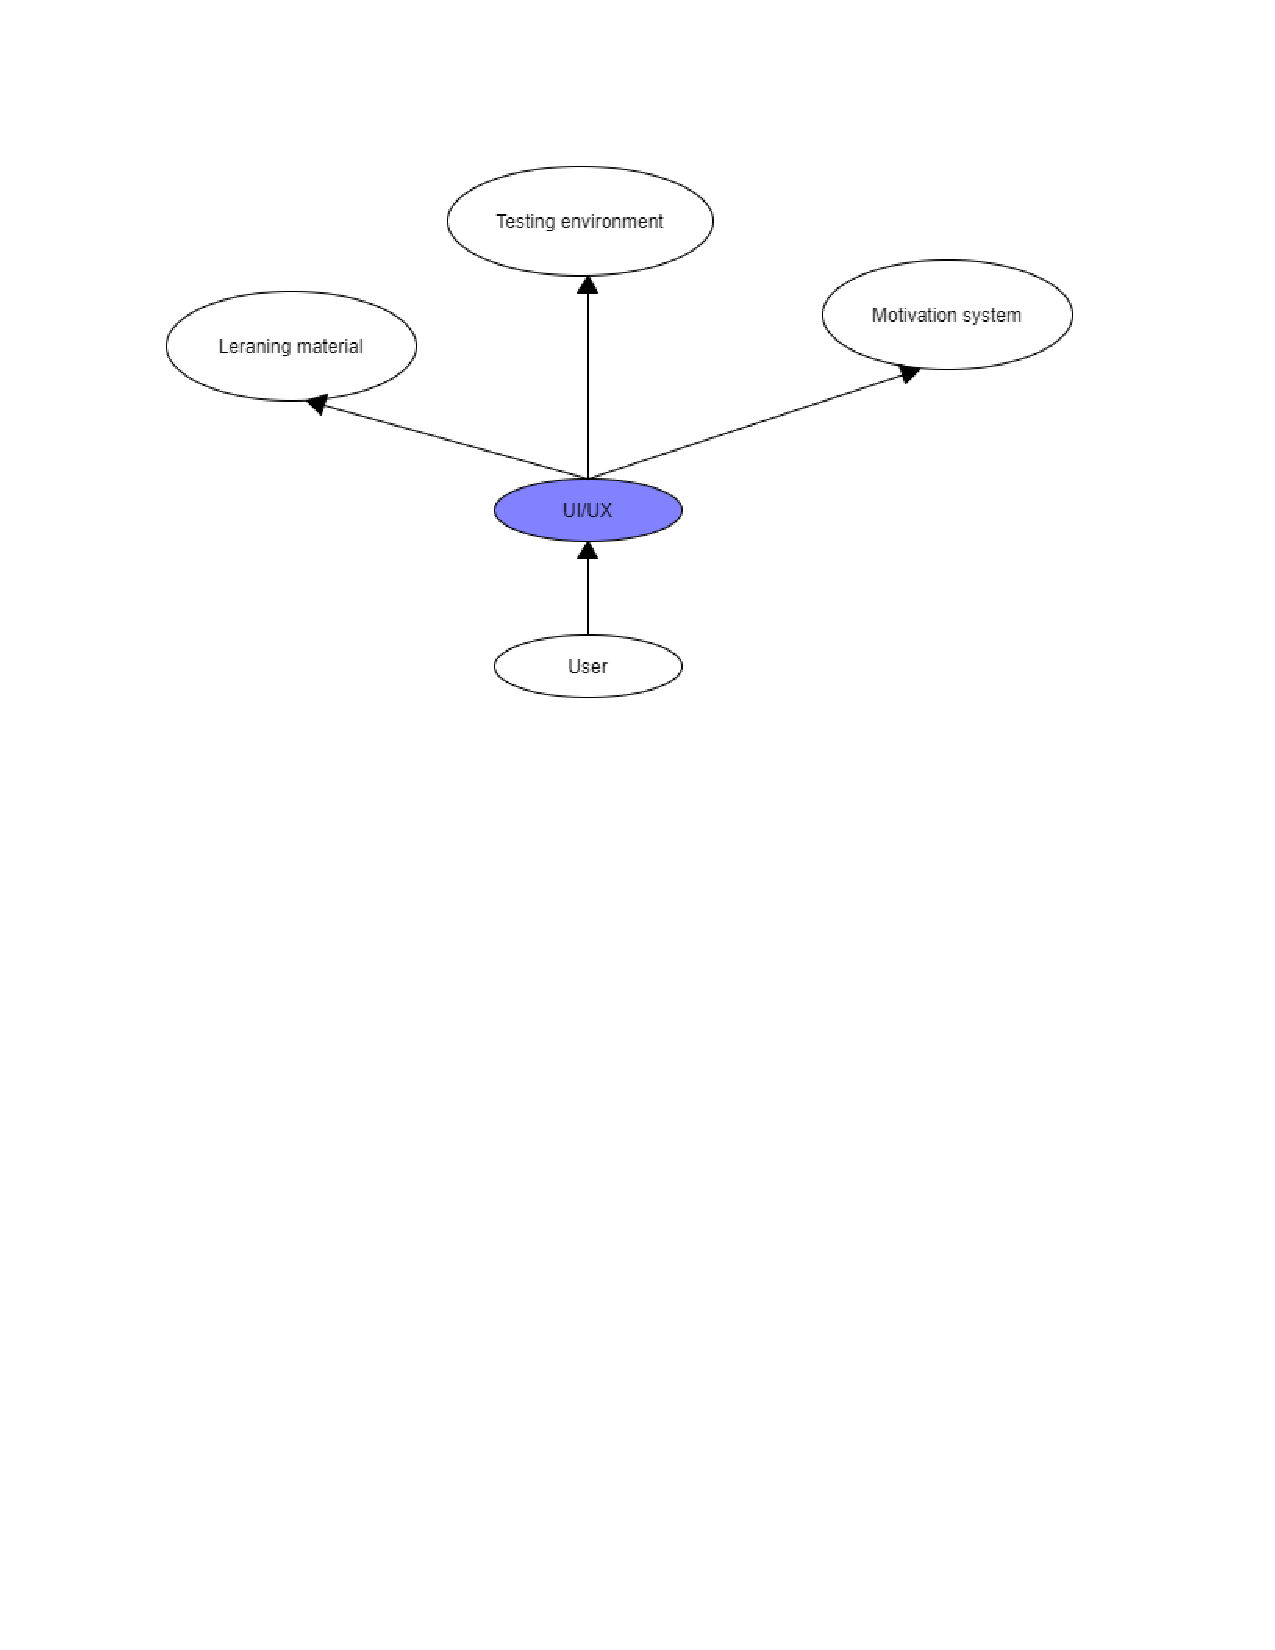
\includegraphics[scale=1.0]{diagram.pdf}
% Aj text môže byť prezentovaný ako obrázok. Stane sa z neho označný plávajúci objekt. Po vytvorení diagramu zrušte znak \texttt{\%} pred príkazom \verb|\includegraphics| označte tento riadok ako komentár (tiež pomocou znaku \texttt{\%}).
% \caption{Rozhodujúci argument.}
% \label{f:rozhod}
% \end{figure*}



% \section{Iná časť} \label{ina}

% Základným problémom je teda\ldots{} Najprv sa pozrieme na nejaké vysvetlenie (časť~\ref{ina:nejake}), a potom na ešte nejaké (časť~\ref{ina:nejake}).\footnote{Niekedy môžete potrebovať aj poznámku pod čiarou.}

% Môže sa zdať, že problém vlastne nejestvuje\cite{Coplien:MPD}, ale bolo dokázané, že to tak nie je~\cite{Czarnecki:Staged, Czarnecki:Progress}. Napriek tomu, aj dnes na webe narazíme na všelijaké pochybné názory\cite{PLP-Framework}. Dôležité veci možno \emph{zdôrazniť kurzívou}.


% \subsection{Nejaké vysvetlenie} \label{ina:nejake}

% Niekedy treba uviesť zoznam:

% \begin{itemize}
% \item jedna vec
% \item druhá vec
% 	\begin{itemize}
% 	\item x
% 	\item y
% 	\end{itemize}
% \end{itemize}

% Ten istý zoznam, len číslovaný:

% \begin{enumerate}
% \item jedna vec
% \item druhá vec
% 	\begin{enumerate}
% 	\item x
% 	\item y
% 	\end{enumerate}
% \end{enumerate}


% \subsection{Ešte nejaké vysvetlenie} \label{ina:este}

% \paragraph{Veľmi dôležitá poznámka.}
% Niekedy je potrebné nadpisom označiť odsek. Text pokračuje hneď za nadpisom.



% \section{Dôležitá časť} \label{dolezita}




% \section{Ešte dôležitejšia časť} \label{dolezitejsia}




% \section{Záver} \label{zaver} % prípadne iný variant názvu



% %\acknowledgement{Ak niekomu chcete poďakovať\ldots}


% týmto sa generuje zoznam literatúry z obsahu súboru literatura.bib podľa toho, na čo sa v článku odkazujete
\bibliography{citations}
\bibliographystyle{plain} % prípadne alpha, abbrv alebo hociktorý iný
\end{document}
